\documentclass{article}
\usepackage[utf8]{inputenc}
\usepackage[T1]{fontenc}
\usepackage{lmodern}
%\renewcommand{\familydefault}{\sfdefault}
%\usepackage{utopia}%\usepackage{XCharter}%\usepackage{beramono}

%writing packages
\usepackage{amsfonts,amsthm,amsmath,amssymb,mathtools,csquotes}
\usepackage{mathrsfs,afterpage,bbm,mdframed}
\usepackage{stix}
\usepackage{epigraph,stmaryrd,xcolor,enumerate}
\usepackage{lipsum}
\usepackage[activate={true,nocompatibility},nopatch=footnote,tracking=true,kerning=true,factor=1100,stretch=10,shrink=10]{microtype}
\microtypecontext{spacing=nonfrench}
\setlength\parindent{0pt}

%graphic packages
\usepackage{tikz,tikz-cd,float,caption,subcaption,graphicx,adjustbox}
\definecolor{pastelred}{rgb}{1.0, 0.41, 0.38}
\definecolor{pastelviolet}{rgb}{0.8, 0.6, 0.79}
\definecolor{pastelgreen}{rgb}{0.47, 0.87, 0.47}
\definecolor{pastelblue}{rgb}{0.47, 0.62, 0.8}
\usepackage{quiver}  
\usepackage{bussproofs}

\usetikzlibrary{decorations.pathmorphing}
\usetikzlibrary{calc}

\let\lrcorner\relax
\newsavebox{\pback} 
\sbox\pback{%
\begin{tikzpicture}%
\draw (0,0) -- (1ex,0ex);%
\draw (1ex,0ex) -- (1ex,1ex);%
\end{tikzpicture}}
\DeclareMathOperator{\lrcorner}{\usebox\pback}

%various packages
\usepackage[
style=alphabetic,
sorting=ynt
]{biblatex}

\addbibresource{bibliography.bib}
\usepackage[english]{babel}
%\usepackage[a-1b]{pdfx}
\usepackage[pdfa]{hyperref}

%Frontespiece packages
\usepackage{subfiles}
\usepackage[a4paper,margin=1.5cm]{geometry}

%commands
\newcommand\myemptypage{
    \null
    \thispagestyle{empty}
    \addtocounter{page}{-1}
    \newpage
    }

\newenvironment{bprooftree}
    {\leavevmode\hbox\bgroup}
    {\DisplayProof\egroup}
\newcommand\tbf[1]{\textbf{#1}}
\newcommand\op[1]{#1^{op}}
\newcommand\co[1]{#1^{co}}
\newcommand\coop[1]{#1^{coop}}
\newcommand{\sbigotimes}{
  \mathop{\mathchoice{\textstyle\bigotimes}{\bigotimes}{\bigotimes}{\bigotimes}}%
}
\newcommand{\sbigoplus}{
  \mathop{\mathchoice{\textstyle\bigoplus}{\bigoplus}{\bigoplus}{\bigoplus}}%
}
\newcommand\sh[1]{\mathcal{#1}}
\newcommand\set[1]{\left\{ #1 \right\}}
\newcommand\shet[1]{\llbracket #1\rrbracket}
\newcommand\bor[1]{\overline{#1}}
\newcommand\mat[1]{\begin{pmatrix}#1\end{pmatrix}}
\newcommand\gen[1]{\left\langle #1 \right\rangle}
\newcommand\tolde[1]{\widetilde{#1}} 
\newcommand\ra[1]{\xsquigrightarrow{#1}}
\newcommand\la[1]{\xsquigleftarrow{#1}}
%numbering settings
\numberwithin{equation}{subsection} 

%theorems
\newtheorem{theorem}[equation]{Theorem}
\newtheorem{proposition}[equation]{Proposition}
\newtheorem{definition}[equation]{Definition}
\newtheorem{observation}[equation]{Observation}
\newtheorem{conjecture}[equation]{Conjecture}
\newtheorem{lemma}[equation]{Lemma}
\newtheorem{corollary}[equation]{Corollary}
\newtheorem*{note}{Note}
\newtheorem*{remark}{Remark}
\newtheorem{example}[equation]{Example}
\newtheorem*{mddd}{Dilly-Dally}
\newenvironment{dd}[1][]%
   {\begin{mdframed}[linecolor=blue]\begin{mddd}[#1]}
   {\end{mddd}\end{mdframed}}
\newtheorem*{exercise}{Exercise}


%operators
\DeclareMathOperator{\Lim}{Lim}
\DeclareMathOperator{\CoLim}{CoLim}
\DeclareMathOperator{\Hom}{Hom}
\DeclareMathOperator{\ob}{ob}
\DeclareMathOperator{\mor}{mor}
\DeclareMathOperator{\Cone}{Cone}
\DeclareMathOperator{\coker}{coker}
\DeclareMathOperator{\im}{im}
\DeclareMathOperator{\coim}{coim}
\DeclareMathOperator{\Mod}{Mod}
\DeclareMathOperator{\eq}{eq}
\DeclareMathOperator{\coeq}{coeq}
\DeclareMathOperator{\Bilin}{Bilin}
\DeclareMathOperator{\End}{End}
\DeclareMathOperator{\subopen}{\subseteq^o}
\DeclareMathOperator{\subclosed}{\bor{\subseteq}}
\DeclareMathOperator{\pre}{pre}
\DeclareMathOperator{\Z}{\mathbb{Z}}
\DeclareMathOperator{\Q}{\mathbb{Q}}
\DeclareMathOperator{\R}{\mathbb{R}}
\DeclareMathOperator{\C}{\mathcal{C}}
\DeclareMathOperator{\A}{\mathbb{A}}
\DeclareMathOperator{\bF}{\mathbb{F}}
\DeclareMathOperator{\N}{\mathbb{N}}
\let\P\relax
\DeclareMathOperator{\P}{\mathbb{P}}
\DeclareMathOperator{\pp}{\mathfrak{p}}
\DeclareMathOperator{\Pp}{\mathcal{P}}
\DeclareMathOperator{\Nn}{\mathscr{N}}
\DeclareMathOperator{\E}{\mathcal{E}}
\DeclareMathOperator{\F}{\mathcal{F}}
\DeclareMathOperator{\G}{\mathcal{G}}
\DeclareMathOperator{\sH}{\mathscr{H}}
\DeclareMathOperator{\I}{\mathscr{I}}
\DeclareMathOperator{\Supp}{Supp}
\DeclareMathOperator{\Ann}{Ann}
\DeclareMathOperator{\Oo}{\mathcal{O}}
\DeclareMathOperator{\Spec}{Spec}
\DeclareMathOperator{\primeideal}{\trianglelefteq_{\mathfrak{p}}}
\DeclareMathOperator{\homogideal}{\trianglelefteq^{\mathcal{H}}}
\DeclareMathOperator{\subaff}{\subseteq^{\text{aff}}}
\let\r\relax
\DeclareMathOperator{\r}{red}
\DeclareMathOperator{\Proj}{Proj}
\DeclareMathOperator{\Frac}{Frac}
\DeclareMathOperator{\Der}{Der}
\DeclareMathOperator{\ch}{char}
\DeclareMathOperator{\ev}{eval}
\let \b\relax
\DeclareMathOperator{\b}{\Box}
\let \d\relax
\DeclareMathOperator{\d}{\Diamond}
\DeclareMathOperator{\Sub}{Sub}
\DeclareMathOperator{\Hull}{Hull}
\DeclareMathOperator{\RelInt}{RelInt}
\DeclareMathOperator{\Fmla}{\textbf{Fmla}}
\DeclareMathOperator{\Log}{\textbf{Log}}
\DeclareMathOperator{\inv}{ inv.}
\DeclareMathOperator{\ar}{ar}
\DeclareMathOperator{\Face}{\textbf{Face}}
\DeclareMathOperator{\Simp}{\textbf{Simp}}
\DeclareMathOperator{\Ll}{\mathcal{L}}
\DeclareMathOperator{\Tr}{Triang}
\newcommand{\upred}{
  \mathrel{\circ}~\kern-0.6em~\relbar\joinrel\twoheadrightarrow
}
\newcommand{\fupred}{
  \mathrel{\circ}~\kern-0.6em~\relbar\joinrel\mapsto
}
%categories
\DeclareMathOperator{\Prop}{\textbf{Prop}}
\DeclareMathOperator{\Uf}{\textbf{Uf}}
\DeclareMathOperator{\PL}{\textbf{PL}}
\DeclareMathOperator{\Sh}{\textbf{Sh}}
\DeclareMathOperator{\Psh}{\textbf{Psh}}
\DeclareMathOperator{\Geom}{\textbf{Geom}}
\DeclareMathOperator{\Top}{\textbf{Top}}
\DeclareMathOperator{\Space}{\textbf{Space}}
\DeclareMathOperator{\Set}{\textbf{Set}}
\DeclareMathOperator{\Grp}{\textbf{Grp}}
\DeclareMathOperator{\Ab}{\textbf{Ab}}
\DeclareMathOperator{\KHaus}{\textbf{KHaus}}
\DeclareMathOperator{\Aa}{\mathcal{A}}
\DeclareMathOperator{\Sch}{\textbf{Sch}}
\DeclareMathOperator{\Ring}{\textbf{CRing}}
\DeclareMathOperator{\LRing}{\textbf{LocRing}}
\DeclareMathOperator{\LRL}{\textbf{LRL}}
\DeclareMathOperator{\Vect}{\textbf{Vect}}
\DeclareMathOperator{\Rel}{\textbf{Rel}}
\DeclareMathOperator{\CAT}{\textbf{CAT}}
\DeclareMathOperator{\CABA}{\textbf{CABA}}
\DeclareMathOperator{\Syn}{\textbf{Syn}}
\DeclareMathOperator{\ASyn}{\textbf{ASyn}}
\DeclareMathOperator{\Cor}{\textbf{Cor}}
\DeclareMathOperator{\Split}{\textbf{Split}}
\DeclareMathOperator{\Pol}{\textbf{Pol}}
\DeclareMathOperator{\Pos}{\textbf{Pos}}
\DeclareMathOperator{\Scplx}{\textbf{Scplx}}

\title{A Goldblatt-Thomason theorem for Compact Polyhedra}
\author{Gabelaia, D. Tognetti, F.}

\begin{document}
\maketitle
\tableofcontents
\section{Polyhedra}
As the title suggests, we are interested in compact polyhedra. Our approach is rooted in the interplay between the geometric and combinatorial facets of these objects, an interplay that is captured most naturally by simplicial complexes.
\subsection{Polyhedra and maps}
\begin{definition}[Simplex]
    Fix a set of \textbf{vertices} $V\subseteq\R^n$ (for some $n\in \N$). For vertices $v_0,\dots,v_k\in V$ in general position (i.e., affinely independent), we say that
    \[\sigma=\set{\sum_{i=0}^k \alpha_i v_i\ |\ \alpha_i\in[0,1],\ \sum\alpha_i=1, v_i\in V}\]
    is a \textbf{face} or \textbf{simplex} with support $v_1,\dots,v_k$.

    For a face $\sigma$ on $v_1,\dots,v_k$, a face whose support is a subset of these vertices is called a \textbf{subface} or \textbf{subsimplex}.

    If a face $\sigma$ has vertices $v_0,\dots,v_k$, we say that $\dim(\sigma)=k$.

    We call $\RelInt(\sigma)$, the \textbf{relative interior} of a face $\sigma$, the interior of the set in the smallest affine subspace of $\R^n$ containing it.
\end{definition}
\begin{definition}[Simplicial complex]
    A \textbf{simplicial complex} is a pair $K=(V,\Sigma)$ where $V$ is a set of vertices and $\Sigma$ is a set of simplices such that
    \begin{itemize}
        \item if $\sigma\in \Sigma$ and $\sigma'$ is a subsimplex of $\sigma$, then $\sigma'\in\Sigma$;
        \item the relative interior of any two simplices is disjoint.
    \end{itemize}
    If $K=(V,\Sigma)$ is a simplicial complex, we say that $\dim(K)=\max_{\sigma\in \Sigma}(\dim(\sigma))$.
\end{definition}

This clearly defines a polyhedron in $\R^n$, but in a way that ``remembers the faces''. We can forget this extra structure and define a polyhedron directly, as follows:

\begin{definition}[Polyhedron]
    Let $K=(V,\Sigma)$ be a simplicial complex. We call
    \[|K|=\bigcup_{\sigma\in\Sigma}\sigma=\bigsqcup_{\sigma\in\Sigma}\RelInt(\sigma)\]
    the \textbf{realization} of $K$, or the \textbf{polyhedron} associated to $K$.

    We say that $P\subseteq \R^n$ is a \textbf{polyhedron} if there exists a simplicial complex $K$ such that $P=|K|$.
\end{definition}

This leads to two notions of maps between polyhedra: one that preserves only the combinatorial structure of the simplicial complex, and one informed by the affine construction above.

\begin{definition}[Simplicial map, PL map]
    Let $K=(V,\Sigma),K'=(V',\Sigma')$ be two geometric simplicial complexes.

    A map $f:|K|\to|K'|$ is called a \textbf{simplicial map} (or \textbf{polyhedral map}) if
    \begin{itemize}
        \item for any point $v\in V$, $f(v)$ is a point of $V'$, and
        \item for any simplex $\sigma\in\Sigma$, $f_{\to}(\sigma)$ is a simplex of $\Sigma'$.
    \end{itemize}

    We further call $f$ \textbf{PL} (\textbf{piecewise linear}) if it is affine when restricted to any face.
\end{definition}

Note that a simplicial complex determines a unique polyhedron, but the converse fails: a polyhedron may be realized by several different simplicial complexes, as in the picture below.
\[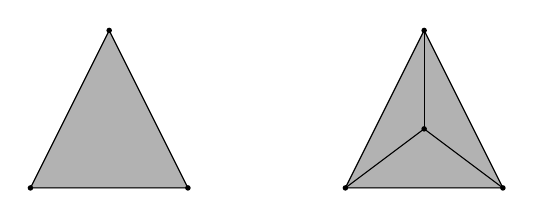
\begin{tikzpicture}[scale=1]
  % Coordinates
  \coordinate (A) at (0.00, 0.00);
  \coordinate (B) at (1.00, 2.00);
  \coordinate (C) at (2.00, 0.00);
  \coordinate (D) at (4.00, 0.00);
  \coordinate (E) at (5.00, 2.00);
  \coordinate (F) at (6.00, 0.00);
  \coordinate (G) at (5.00, 0.75);

  % Drawing
  \draw (A) -- (B) -- (C) -- cycle;
  \draw (D) -- (E) -- (F) -- cycle;
  \draw[fill,opacity=0.3] (A) -- (B) -- (C) -- cycle;
  \draw[fill,opacity=0.3] (D) -- (E) -- (F) -- cycle;
  \draw (G) -- (E);
  \draw (D) -- (G);
  \draw (F) -- (G);
  \fill[black] (A) circle (1pt);
  \fill[black] (B) circle (1pt);
  \fill[black] (C) circle (1pt);
  \fill[black] (D) circle (1pt);
  \fill[black] (E) circle (1pt);
  \fill[black] (F) circle (1pt);
  \fill[black] (G) circle (1pt);
\end{tikzpicture}\]
In the picture above, the two polyhedra are clearly the same (a triangle), but the complex on the left has a single face of dimension $2$, while the complex on the right has three.
\begin{definition}[Triangulation]
    Let $P$ be a polyhedron in $\R^n$. A simplicial complex $K$ such that $|K|=P$ is called a \textbf{triangulation} of $P$.
\end{definition}

In particular, starting from a single simplicial complex, we can generate arbitrarily rich simplicial complexes that all realize the same polyhedron.
\begin{definition}[Barycentric subdivision]
    Recall that if $\sigma=\set{\sum_{i=0}^k \alpha_i v_i\ |\ \alpha_i\in[0,1],\ \sum\alpha_i=1, v_i\in V}$, the point
    \[b_\sigma=\frac{1}{k+1}\sum_{i=0}^k v_i\]
    is called the \textbf{barycenter} of $\sigma$.

    Let $K=(V,\Sigma)$ be a simplicial complex. We call the \textbf{barycentric subdivision} of $K$ the simplicial complex $K^{(1)}$ having as vertices the set of barycenters of faces in $\Sigma$,
    \[V^{(1)}=\set{b_\sigma:\sigma\in\Sigma}\]
    and as simplices those obtained by inductively replacing vertices with barycenters, in decreasing order of dimension:
    \[\sigma^{(1)}_{j}=\set{\alpha_1 v_1+\cdots+\widehat{\alpha_j v_i}+\alpha_j b_{\sigma}+\cdots+\alpha_k v_k\ |\ \alpha_i\in[0,1],\ \sum\alpha_i=1}\]
\end{definition}
Visually, the barycentric subdivision of a triangle looks as follows:
\[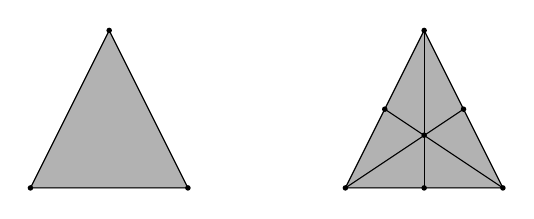
\begin{tikzpicture}[scale=1]
  % Coordinates
  \coordinate (A) at (0.00, 0.00);
  \coordinate (B) at (1.00, 2.00);
  \coordinate (C) at (2.00, 0.00);
  \coordinate (D) at (4.00, 0.00);
  \coordinate (E) at (5.00, 2.00);
  \coordinate (F) at (6.00, 0.00);
  \coordinate (G) at (5.00, 0.67);
  \coordinate (H) at (5.00, 0.00);
  \coordinate (I) at (5.50, 1.00);
  \coordinate (J) at (4.50, 1.00);

  % Drawing
  \draw (A) -- (B) -- (C) -- cycle;
  \draw (D) -- (E) -- (F) -- cycle;
  \draw[fill,opacity=0.3] (A) -- (B) -- (C) -- cycle;
  \draw[fill,opacity=0.3] (D) -- (E) -- (F) -- cycle;
  \draw (H) -- (E);
  \draw (D) -- (I);
  \draw (F) -- (J);
  \fill[black] (A) circle (1pt);
  \fill[black] (B) circle (1pt);
  \fill[black] (C) circle (1pt);
  \fill[black] (D) circle (1pt);
  \fill[black] (E) circle (1pt);
  \fill[black] (F) circle (1pt);
  \fill[black] (G) circle (1pt);
  \fill[black] (H) circle (1pt);
  \fill[black] (I) circle (1pt);
  \fill[black] (J) circle (1pt);
\end{tikzpicture} \]

\begin{theorem}[$|K|=|K^{(1)}|$]
    The geometric realization of a simplicial complex is unchanged by barycentric subdivision.
\end{theorem}
\begin{proof}
    We must show two inclusions: that $\sigma_j^{(1)}\subseteq \sigma$ for all $\sigma$ and all $j$, and that $\sigma\subseteq \bigcup_j\sigma^{(1)}_j$.

    For the first claim, suppose $p\in\sigma_j^{(1)}$; without loss of generality, $p\in \sigma_1^{(1)}$. Then
    \begin{align*}
        p&=a_1 b_\sigma + a_2 v_2+\cdots + a_kv_k\\
        &=\frac{a_1}{k+1}(v_1+\cdots+v_k)+a_2v_2+\cdots+a_kv_k\\
        &=\frac{a_1}{k+1} v_1+ (a_2+\frac{a_1}{k+1})v_2+\cdots+(a_k+\frac{a_1}{k+1})v_k.
    \end{align*}
    Now
    \begin{align*}
        &\frac{a_1}{k+1}+(a_2+\frac{a_1}{k+1})+\cdots+(a_k+\frac{a_1}{k+1})\\
        &=(k+1)\frac{a_1}{k+1}+a_2+\cdots+a_k\\
        &=a_1+a_2+\cdots+a_k=1,
    \end{align*}
    and all of these coefficients are positive. This means that any subdivision obtained by replacing a vertex with the barycenter of a face containing it, and taking the convex hull, is contained in the original face. Since the barycentric subdivision is an iteration of this process, $K^{(1)}\subseteq K$.

    For the converse, suppose $p\in \sigma$, so that
    \[p=a_1v_1+\cdots+a_kv_k.\]
    We want to find $b_1,\dots,b_k$ such that $p=b_1 v_1 + \cdots + b_j b_\sigma +\cdots + b_k v_k$. Substituting backwards,
    \begin{align*}
        &b_j v_j + b_1 v_1 + \cdots + b_k v_k\\
        &=\frac{a_j}{k+1} v_j + (a_1+\frac{a_j}{k+1}) v_1 + \cdots + (a_k+\frac{a_j}{k+1}) v_k,
    \end{align*}
    which yields the system of equations
    \[a_j=(k+1)b_j,\quad a_1= b_1-b_j, \quad \cdots, \quad a_k=b_k-b_j.\]
    To ensure that all the $b_i$ are positive, we choose $j$ to realize the minimum of the $b_j$.

    An induction on the subdivision then gives $K\subseteq K^{(1)}$.
\end{proof}
\subsection{Posets}
Forgetting the support in $\R^n$ gives a purely combinatorial description of a simplicial complex: what remains is essentially a downward-closed poset.
\begin{definition}[Face poset]
    Let $K=(V,\Sigma)$ be a simplicial complex. We call $[K]=(\Sigma,\subseteq)$ the \textbf{face poset} of $K$.
\end{definition}

The face poset $[K]$ already contains everything we need to recover the structure of $K$ up to PL-homeomorphism.
\begin{lemma}
    Let $K,K'$ be two simplicial complexes with $[K]\simeq [K']$. Then there exists a PL-homeomorphism $K\simeq K'$.
\end{lemma}
\begin{proof}
    See \cite[Lemma 2.18]{PLTopology}.
\end{proof}

This allows us to define:
\begin{definition}[ASC]
    An \textbf{abstract simplicial complex}, or \textbf{ASC}, is a pair $K=(V,\Sigma)$ where $V$ is a set and $\Sigma\subseteq \Pp(V)$ is a collection of subsets of $V$ closed under taking subsets.

    Given a simplicial complex $K$, associating to each face the set of its vertices yields an ASC $\overline{K}$.
\end{definition}

Conversely, every ASC arises this way from an essentially unique simplicial complex.
\begin{lemma}
    Let $K$ be an ASC. Then there exists a simplicial complex $K'$ such that $\overline{K'}=K$.
\end{lemma}
\begin{proof}
    Realize every $d$-simplex as the standard simplex of the appropriate dimension in $\R^{d+1}$, and glue them together according to their intersections; see \cite{PLTopology} for a complete account.
\end{proof}
Together, these two lemmas give a correspondence
\[\dfrac{\set{\textbf{Simplicial Complexes}}}{\text{PL-homeomorphism}}\leftrightarrow\set{\textbf{ASCs}}\]
since to each ASC we may associate a simplicial complex, and any two simplicial complexes associated to the same ASC are PL-homeomorphic.

We also want a way to define an (abstract) simplicial complex from any poset:

\begin{definition}[Nerve]
    Let $(P,\leq)$ be a poset. We call $\Nn(P)$, the \textbf{nerve} of $P$, the abstract simplicial complex whose vertices are the elements of $P$ and whose simplices are the flags $p_1<\cdots<p_k$ of ordered elements of $P$.
\end{definition}

We will freely use the following fact:
\begin{theorem}
    If $K=(V,\Sigma)$ is a simplicial complex, then
    \[\Nn(\Sigma)=\overline{K^{(1)}}.\]
\end{theorem}
\begin{proof}
    See \cite{PLTopology}.
\end{proof}
\subsection{Subdivision theorems}
We are interested in polyhedra as semantics for modal logic, and so our choice of morphisms differs slightly from the classical framework.

Recall first that, given (binary) Kripke frames $(W,R)$ and $(W',R')$, a function $f:W\to W'$ is called a p-morphism if and only if it satisfies
\begin{enumerate}
    \item $w R w'$ implies $f(w) R f(w')$;
    \item $f(v) R w'$ implies that there exists $w\in W$ such that $v R w$ and $f(w)=w'$.
\end{enumerate}

If $R=\leq$ is a partial order, these two conditions become equivalent to
\[\forall w\in W.\ \uparrow f(w)=f(\uparrow w),\]
where $\uparrow w=\set{v\in W: w<v}$. We refer to this property as \textbf{upward-closure}.

The proofs of all the following lemmas can be found in \cite{Dekker}.
\begin{lemma}[Subdivisions are p-morphic]
    The map $K^{(1)}\twoheadrightarrow K$ sending each face of $\Sigma^{(1)}$ to the (unique) face of $\Sigma$ containing it is a p-morphism.
\end{lemma}
\begin{lemma}[Common triangulation]
    Let $K$ be a simplicial complex and $K'\subseteq K$ another simplicial complex. Then there exists a subdivision $L$ of $K$, and a subset $L'$ of $L$ that is a subdivision of $K'$.
\end{lemma}
This is easy to visualize:
\[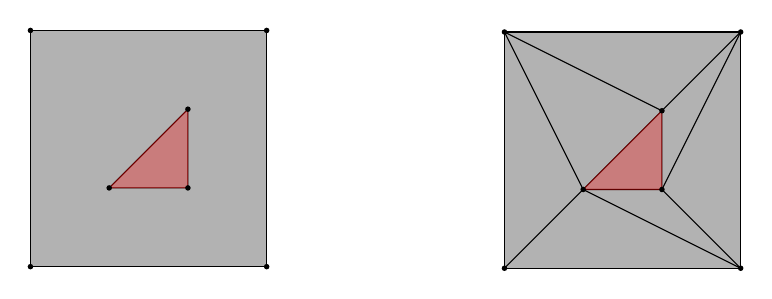
\begin{tikzpicture}[scale=1]
  % Coordinates
  \coordinate (A) at (0.00, 0.00);
  \coordinate (B) at (0.00, 3.00);
  \coordinate (C) at (3.00, 3.00);
  \coordinate (D) at (3.00, 0.00);
  \coordinate (E) at (1.00, 1.00);
  \coordinate (F) at (2.00, 2.00);
  \coordinate (G) at (2.00, 1.00);
  \coordinate (H) at (6.02, -0.02);
  \coordinate (I) at (6.02, 2.98);
  \coordinate (J) at (9.02, 2.98);
  \coordinate (K) at (9.02, -0.02);
  \coordinate (L) at (7.02, 0.98);
  \coordinate (M) at (8.02, 1.98);
  \coordinate (N) at (8.02, 0.98);

  % Drawing
  \draw (A) -- (B) -- (C) -- (D) -- cycle;
  \draw[fill, opacity=0.3] (A) -- (B) -- (C) -- (D) -- cycle;
  \draw (E) -- (F) -- (G) -- cycle;
  \draw[red,fill, opacity=0.3] (E) -- (F) -- (G) -- cycle;
  \draw (H) -- (I) -- (J) -- (K) -- cycle;
  \draw[fill, opacity=0.3] (H) -- (I) -- (J) -- (K) -- cycle;
  \draw (L) -- (M) -- (N) -- cycle;
  \draw[red,fill, opacity=0.3]  (L) -- (M) -- (N) -- cycle;
  \draw (H) -- (L);
  \draw (L) -- (K);
  \draw (N) -- (K);
  \draw (N) -- (J);
  \draw (M) -- (J);
  \draw (M) -- (I);
  \draw (L) -- (I);
  \fill[black] (A) circle (1pt);
  \fill[black] (B) circle (1pt);
  \fill[black] (C) circle (1pt);
  \fill[black] (D) circle (1pt);
  \fill[black] (E) circle (1pt);
  \fill[black] (F) circle (1pt);
  \fill[black] (G) circle (1pt);
  \fill[black] (H) circle (1pt);
  \fill[black] (I) circle (1pt);
  \fill[black] (J) circle (1pt);
  \fill[black] (K) circle (1pt);
  \fill[black] (L) circle (1pt);
  \fill[black] (M) circle (1pt);
  \fill[black] (N) circle (1pt);
\end{tikzpicture}\]

\begin{lemma}[Nerves are dense]
    Let $K$ be a simplicial complex and $L$ a subdivision of $K$.

    Then there exists $n\in \N$ such that $K^{(n)}$ is (isomorphic to) a subdivision of $L$.
\end{lemma}

\begin{lemma}[Subdividing p-morphisms]
    Let $K,K'$ be simplicial complexes and $f:K\upred K'$ an up-reduction, that is, a p-morphism defined on an upward-closed (open) subset of $K$.

    Let $L'$ be a subdivision of $K'$. Then there exists a subdivision $L$ of $K$ and an up-reduction $L\upred L'$ such that

    \[\begin{tikzcd}[ampersand replacement=\&]
	K \& {K'} \\
	L \& {L'}
	\arrow["\circ"{description, pos=0.17}, from=1-1, to=1-2, two heads]
	\arrow[from=2-1, to=1-1]
	\arrow["\circ"{description, pos=0.17}, from=2-1, to=2-2, two heads]
	\arrow[from=2-2, to=1-2]
\end{tikzcd}\]
\end{lemma}

\section{Definability}
Here we render explicit the standard (Kripke) version of our definability theorem, explain our choice of semantics, 
and suggest how we will transport the standard result to the new setting.

\subsection{Polyhedral semantics}
As is always the case, we begin with a syntax: here we consider the standard propositional modal language.
\begin{definition}[Modal language]
    Our language is the standard modal language: 
    we assume a set of propositional variables $X$ 
    and define inductively
    \[\Ll = \set{x\in X \ \|\ \bot\ \|\ \varphi\vee\psi\ \|\ \lnot\varphi\ \|\ \d\varphi}\]
\end{definition}
This is a minimal description of our syntax, 
where we can assume the ``not'' to be primitive and derive 
\begin{itemize}
    \item $\top=\lnot\bot$
    \item $\varphi \wedge \psi=\lnot(\lnot \varphi\vee\lnot\psi)$
    \item $\varphi\to\psi=\lnot \varphi\vee\psi$
    \item $\b \varphi=\lnot\d\lnot\varphi$
\end{itemize}
Our semantics is a tamer version of the topological 
semantics for modal logic (\cite{Gabelaia2001ModalDI}), 
interpreting the box $\b$ as an interior operator
and the diamond $\d$ as a closure operator.

The main difference between polyhedral and topological semantics 
is that the evaluations of the elementary propositions are 
(possibly open) subpolyhedra and not arbitrary subsets.

Recall that a subpolyhedron (\ref{Polyhedron}) is a union of relative interiors of subsimplices.

\begin{definition}[Polyhedral semantics]
    Let $P$ be a (compact) polyhedron. An \textbf{evaluation} is a map $\nu :\Ll \to \Pp(P)$ such that $\nu(\varphi)$ is a union of relative interiors of subpolyhedra of $P$.

    Moreover, we ask that $\nu$ satisfies the following properties:
    \begin{itemize}
        \item $\nu(\bot)=\emptyset$,
        \item $\nu(\varphi\vee\psi)=\nu(\varphi)\cup\nu(\psi)$,
        \item $\nu(\lnot\varphi)=P\setminus \nu(\varphi)$,
        \item $\nu(\d\varphi)=\overline{\nu(\varphi)}$.
    \end{itemize}
    We say $P,x\models \varphi$ if and only if $x\in \nu(\varphi)$, 
    and we say that $\varphi$ \textbf{is valid in} $P$, 
    written $P\models\varphi$, if $P,x\models \varphi$ 
    for every $x\in P$ and every evaluation $\nu$.
\end{definition}

This allows us to define the \textbf{logic} of a polyhedron, i.e. the set of formulas that are valid in a given polyhedron.
\begin{definition}
    Let $P$ be a polyhedron. We call the \textbf{logic} of $P$ the set
    \[\Log(P):=\set{\varphi\in \Ll:P\models\varphi}\]
\end{definition}

Recall that the Kripke semantics for the modal logic (S4.Grz) interprets the Boolean connectives as usual, together with
\[P,p\models \d\varphi\iff \exists q\geq p: P,q\models\varphi.\]
($\d \varphi$ is true at $p$ if and only if $\varphi$ is true on some element above $p$).

The following theorem connects the two semantics:
\begin{theorem}
    Let $P$ be a polyhedron and let $K=(V,\Sigma)\in \Tr(P)$ be a simplicial complex realizing $P$.

    For each $x\in P$ there exists a unique $\sigma_x\in \Sigma$ such that $x\in \RelInt(\sigma_x)$, and
    \[P,x\models\varphi \text{ (as polyhedra) if and only if }\Sigma,\sigma_x\models\varphi\text{ (as posets)}.\]
    Moreover,
    \[\Log(P)=\bigcap_{K\in \Tr(P)}\Log([K]).\]
\end{theorem}
\begin{proof}
    See \cite{TENCATE} and \cite{DBLP} for a complete account.
\end{proof}

In the form of a slogan: a formula is satisfied on a polyhedron if and only if it's satisfied on some triangulation,
and a formula is valid on a polyhedron if and only if it's valid on every triangulation.

\subsection{Modally definable classes}

The dual question to validity is definability: given a set of formulas $F$, we can define the class of models validating it:

\begin{definition}[Modally definable class]
    \label{MD1}
    Let $F\subseteq \Ll$ be a set of formulas. We call $\Pol(F)$ the class of (compact) polyhedra modeling every formula of $F$, i.e.
    \[\Pol(F)=\set{P\in\Pol: \forall\varphi\in F. P\models\varphi}\]
\end{definition}

Goldblatt and Thomason's theorem gives necessary and sufficient condition for when an arbitrary class of frames $\C$ is modally definable, i.e. 
it is the class of models validating some set of formulas.

Every flavor of models generates a slightly different Goldblatt-Thomason-like theorem. The classical result about 
frames states that a class of Kripke frames is modally definable if and only if it's closed under disjoint unions,
generated subframes, p-morphic images and it's closed under and reflects ultrafilter extensions.

Here we recall
\begin{definition}[Generated subframe]
    Let $(W,R)$ be a frame, $V\subseteq W$ is called a \textbf{generated subframe}
    if and only if it's upward-closed, i.e. for any $v\in V, $ if $vRv'$ then $v'\in V$ too.

    When $R=\leq$ this translates to the usual notion of upward closure.
\end{definition}

As we are considering compact polyhedra, our frames (posets) are finite, thus we can use a stronger theorem with easier conditions.

\begin{theorem}[Goldblatt-Thomason for finite transitive frames (I)]
    \label{GTFT1}
    A class of finite transitive frames $\C$ is modally definable if and only if it is closed under
    \begin{enumerate}
        \item finite disjoint unions,
        \item generated subframes,
        \item p-morphic images.
    \end{enumerate}
\end{theorem}
\begin{proof}
    See \cite{Blackburn_Rijke_Venema_2001}, Chapter 3.
\end{proof}

We see that generated subframes correspond to open subpolyhedra. This constitute a problem: Our polyhedra lay in some euclidean space, thus have open non-compact subsets.

Such a subset cannot be part of our class as it's not compact, but a priori there might be maps that can be defined on it and not on the starting space.

Our solution is to avoid considering generated subframes (equivalently open subpolyhedra) and combine the notion of generated subframe and p-morphic image into one notion.

We need to show equivalence, so let us state it as a corollary and prove it.
\begin{corollary}[Goldblatt-Thomason for finite transitive frames (II)]
    A class of finite transitive frames $\C$ is modally definable if and only if it is closed under
    \begin{enumerate}
        \item finite disjoint unions,
        \item[(3')] surjective up-reductions,
    \end{enumerate}
\end{corollary}
\begin{proof}
    Suppose $\C$ is closed under the conditions (1),(2), and (3) of \ref{GTFT1}. Let $X\in \C$ and let $f:X\upred Y$ be an up-reduction. As an up-reduction is a partial function, call $U$ 
    the domain of definition of $f$. Thanks to condition (2) we know that $U\in \C$.

    Then $f_{|U}: U\twoheadrightarrow Y$ is a surjective p-morphism, 
    so $Y$ is a p-morphic image of $U$, and thus by (3) $Y\in \C$. 
    This means that $\C$ is closed under (3').

    Conversely, suppose that $\C$ is closed under (1) and (3'). 
    Let $X\in \C$ and let $U$ be a generated subframe of 
    $X$. Then the identity on $U$, 
    seen as a partial map $X\to U$, is an up-reduction. 
    Similarly, if $Y$ is a p-morphic image of $Y$, then, 
    since $X$ is a generated subframe of $X$, we may extract an up-reduction $X\upred Y$.
\end{proof}

Note that this means the class of frames is always closed under generated subframes, but we may consider this class within a category that lacks them.

We will also make use of the Jankov-Fine axiomatization: There exists some formulas that prohibit up-reduction to a given (rooted) frame, i.e. a model validates 
the formula corresponding to the frame if and only if it does not up-reduce to the frame.

These formulas are useful for example and counterexamples and fully characterize classes of finite frames.

\begin{theorem}[Jankov-Fine]
    Let $U$ be a finite rooted frame. Then there exists a formula $\chi(U)$ such that $F\models\chi(U)$ if $F$ does \textbf{not} up-reduce to $U$.
\end{theorem}
\begin{proof}
    See \cite{Bezhanishvili2022}.%provide a more direct source?
\end{proof}
\begin{corollary}
    A class of finite frames $\C$ can be characterized as
    \[\C=\Mod(\set{\chi(U)\ |\ U\notin \C,\ U \text{ rooted}}).\]
\end{corollary}


\section{GTKP}
\subsection{Face up-reductions}
To any poset we can assign a topology compatible with the topological semantics.

\begin{definition}[Alexandrov topology]
    Let $(P,\leq)$ be a poset. We call the \textbf{Alexandrov} topology on $P$ the collection $\tau\subseteq \Pp P$ where $U\in\tau$ if and only if $U$ is upward-closed.
\end{definition}

We use it to define a weaker version of the up-reduction between polyhedra.
\begin{definition}[Face up-reduction]
    Let $P,Q$ be (compact) polyhedra and $K$ a triangulation of $Q$.

    A \textbf{face up-reduction} $P\fupred Q$ is a partial map $f:P\upred [K]$ such that
    \begin{enumerate}[(i)]
        \item the preimage of every open of $[K]$ (in the Alexandrov topology) is an open subpolyhedron of $P$;
        \item it is \textbf{open};
        \item it is \textbf{surjective}.
    \end{enumerate}
\end{definition}

We note the following:
\begin{proposition}
    $Q\upred[K]$ for any triangulation $K$.

    In particular, $Q\fupred Q$.
\end{proposition}
\begin{proof}
    Let $K$ be a triangulation of $Q$, and let $f$ be the map $q\mapsto \sigma_q$, where $\sigma_q$ is the unique face of $K$ such that $q\in\sigma_q$. Since every point of $Q$ lies in a unique such face, $f$ is trivially surjective.

    Note that the preimage of a face $\sigma$ is the corresponding face of the polyhedron, $f^{\gets}(\sigma)=|\sigma|$.

    If $U$ is an upward-closed subset of $[K]$, then $[K]\setminus U$ is downward-closed, and hence is a compact polyhedron. This means that $f^\gets([K]\setminus U)=Q\setminus f^{\gets}(U)$ is compact, and hence closed; therefore $f^\gets(U)$ is open and is a union of faces, i.e., an open subpolyhedron.

    This same argument shows that the map is open: if $P\subseteq Q$ is an open subpolyhedron, then $Q\setminus P$ is a compact polyhedron, so $[K]\setminus f(P)$ is downward-closed, so $f(P)$ is upward-closed, i.e., open.
\end{proof}
\begin{corollary}
    If there exists an up-reduction, i.e., an open partial simplicial map $P\upred Q$ whose domain is an open subpolyhedron of $P$, then $P\fupred Q$.
\end{corollary}


We may also make explicit the following fact:

\begin{lemma}
    Let $f:P\fupred Q$ be a face up-reduction, let $U\subseteq^o P$ be its domain, and let $L$ be the triangulation of $Q$ such that $f:U\upred [L]$.

    Then there exists a triangulation $K$ of $P$ such that
    \begin{itemize}
        \item $U$ is the union of relative interiors of faces of $K$, i.e. $U=\bigcup_{\sigma\in K_U}\RelInt\sigma$.
        \item $\tilde{f}:[K]\upred[L]$ defined as $\tilde{f}(\sigma_p)=f(p)$ is an up-reduction of posets.
    \end{itemize}
\end{lemma}
\begin{proof}
    Note that $[L]$ is a \textbf{finite} poset and that $\set{f^\gets(l):l\in L}$ is a collection of possibly open polyhedra in $P$. By the common triangulation lemma, we may extract a common triangulation $K$ of all of them.

    Now, recall that for each point $p\in P$ there exists a unique face $\sigma_p$ such that $p\in\RelInt(\sigma_p)$. This allows us to define $\tilde{f}$ as above. Uniqueness ensures that $\tilde{f}$ is well-defined, and openness of $f$ gives $f(\uparrow\sigma_p)=\uparrow f(p)$.
\end{proof}
\begin{lemma}[Up-reductions refute formulas]
    Let $P$ be a polyhedron, $S$ a poset, and $P\upred S$ an up-reduction.

    If $S\not\models \varphi$, then $P\not\models\varphi$ as well.
\end{lemma}
\begin{proof}
    The proof proceeds essentially as in the topological case in \cite{Gabelaia2001ModalDI}.
\end{proof}

\subsection{Goldblatt-Thomason for compact polyhedra}
\begin{theorem}[GTKP]
    A class of compact polyhedra $\C$ is modally definable if and only if it is closed under finite disjoint unions and face up-reductions, i.e.,
    \begin{enumerate}[(I)]
        \item if $P,Q\in \C$, then $P\sqcup Q\in \C$;
        \item if $P\in \C$ and $P\fupred X$, then $X\in \C$.
    \end{enumerate}
\end{theorem}
\begin{proof}[Proof ($\implies$)]
    Let $\C$ be a modally definable class, i.e., $\C=\set{P\in \Pol:P\models F}$ for some set of formulas $F$.

    Closure under disjoint union is trivial: if $P,Q\in \C$, then $P\sqcup Q\models F$.

    Suppose $P\in \C$ and $P\fupred X$, and suppose toward a contradiction that $X\notin \C$. By definition, this means that there exists a formula $\varphi\in F$ such that $X\not\models\varphi$.

    Spelling out the validity condition, there exists an evaluation $\nu:\Ll\to \Pp X$ and a point $x\in X$ such that $X,x\not\models\varphi$.

    By the common triangulation lemma, we may select a triangulation $S$ of $X$ such that $\nu(\varphi)$ is triangulated by $S$.

    Call $K=(V,\Sigma)$ the triangulation of $X$ realizing the face up-reduction $P\fupred X$. By the `nerves are dense' lemma, there exists a barycentric subdivision $K^{(n)}$ of $K$ subdividing $S$.

    We also know that we can extend any up-p-morphism $P\upred \Sigma$ to an up-p-morphism $P\upred \Sigma^{(k)}$, for any $k\in \N$.

    This gives an up-p-morphism $P\upred \Sigma^{(k)}\upred S$, and therefore $P\not\models\varphi$ --- a contradiction.
\end{proof}
\begin{proof}[Proof ($\impliedby$)]
    Let $\C$ be a class of polyhedra closed under (I) and (II); call $L:=\Log(\C)$ and $\C'=\Pol(L)$.

    Clearly $\C\subseteq \C'$. Let $X\in \C'$; we want to show that $X\in \C$.

    We know that $X\models L$; let $K=(V,\Sigma)\in \Tr(X)$ and call $v_i$ the vertices of $\Sigma$. We know that
    \[\bigsqcup_i (\uparrow v_i)\twoheadrightarrow \Sigma\]
    is a p-morphism.

    Consider $\chi_i:=\chi(\uparrow v_i)$, the Jankov-Fine formula for the (rooted) subposet $\uparrow v_i$.

    Since $(\uparrow v_i)\not\models \chi_i$, and each $(\uparrow v_i)$ is a generated subframe of $\Sigma$, we know that $\Sigma\not\models\chi_i$.

    In particular $X\upred\Sigma$, and thus $X\not\models\chi_i$ for all $i$. This means that none of the $\chi_i$ belong to $L$, so for each $\chi_i$ there exists some $P_i\in \C$ such that $P_i\not\models \chi_i$, and thus $P_i\upred(\uparrow v_i)$.

    It follows that $P:=\bigsqcup_i P_i$ admits an up-p-morphism to $\bigsqcup_i(\uparrow v_i)$; composing with $\bigsqcup_i(\uparrow v_i)\twoheadrightarrow \Sigma$ yields an up-reduction $P\upred \Sigma$, and hence a face up-reduction $P\fupred X$.

    By (I), $P\in \C$, and by (II), $X\in \C$.
\end{proof}

\begin{corollary}
    A class of polyhedra closed under finite disjoint unions and simplicial up-reductions is modally definable, where a simplicial up-reduction is an open simplicial partial map $f:P\upred Q$ whose domain is an open subpolyhedron of $P$.
\end{corollary}
\begin{proof}
    This follows from Corollary 3.1.4: if $f:P\upred Q$ is a simplicial up-reduction, then there exists a face up-reduction $P\fupred Q$ by composing with the face p-morphism onto any face poset.
\end{proof}

The theorem above can be strengthened by the following lemma.
\begin{lemma}[Any triangulation]
    Suppose $P\upred \Sigma$ is an up-reduction, for a triangulation $L=(V,\Sigma)$ of $Q$, and let $L'=(V',\Sigma')$ be a different triangulation of $Q$. Then there also exists an up-reduction $P\upred \Sigma'$.
\end{lemma}
\begin{proof}
    Let $f:P\upred\Sigma$ be an up-reduction with domain $U\subseteq P$. We extend $f$ to $f^{(1)}:P\upred\Sigma^{(1)}$ as follows.

    Take the triangulation $K$ of $P$ realizing $f$ as a simplicial map $\tilde{f}$ (Lemma 3.1.5), and use the subdivision lemma (Lemma 1.3.4) to extract an up-reduction $K'\upred L^{(1)}$.

    Now, repeatedly applying Lemma 1.3.3, we may iterate this $n$ times so that $L^{(n)}$ is a subdivision of $L'$. This gives a map $h: K^{\prime \cdots\prime }\upred L^{(n)}\twoheadrightarrow L'$.

    Since $K^{\prime \cdots\prime }$ is a triangulation of $P$, we can extract an up-reduction $g:P\upred L'$ by setting it to be locally constant on the relative interior of each face of $P$.
\end{proof}

In other words, if a face up-reduction exists to one triangulation, then one exists to any triangulation, even with the same domain.

\section{Applications}
\subsection{Some modally definable classes}
We start by giving some fairly obvious examples of modally definable classes.

Recall that 
\[\Pol(F)\coloneqq \set{P\in\Pol:P\models F}\]

And some standard formulas: 
\begin{definition}$ $\\
    \begin{itemize}
        \item Grz (the Grzegorczyk formula): \[\b(\b(\varphi\to\b\varphi)\to\varphi)\to \varphi\]
        \item Bd$_n$ is the Jankov-Fine formula of the linear order of length $n+1$ 
        \[\text{Bd}_n=\chi(\bullet - \bullet -\cdots -\bullet)\]
        \item $F_n$ (the $n-$fork) is the poset with a single root and $n$ leaves only connected to the root.
    \end{itemize}
\end{definition}
\begin{figure}[H]
    \centering 
    \begin{tikzcd}[ampersand replacement=\&,scale=0.5]
	\bullet \& \bullet \& \bullet \&\& \bullet \& \bullet \& \bullet \& \bullet \& \bullet \\
	\& \bullet \& {F_3} \&\&\&\& \bullet \&\& {F_5}
	\arrow[no head, from=1-1, to=2-2]
	\arrow[no head, from=1-2, to=2-2]
	\arrow[no head, from=1-3, to=2-2]
	\arrow[no head, from=1-5, to=2-7]
	\arrow[no head, from=1-6, to=2-7]
	\arrow[no head, from=1-7, to=2-7]
	\arrow[no head, from=1-8, to=2-7]
	\arrow[no head, from=1-9, to=2-7]
\end{tikzcd}
\caption{A visual representation of the $3-$fork and the $5-$fork}
\end{figure}
\begin{proposition}[Bounded dimension]
    For any given $n\in\N$, the class of polyhedra of dimension
    $\leq n$ is modally definable.
\end{proposition}
\begin{proof}
    Indeed, it is $\Pol(S4.\text{Grz}.\text{Bd}_n)$.
    It was shown in previous works (\cite{DBLP,Dekker}) that a polyhedron has dimension 
    less or equal to $n$ if and only if it validates the bounded depth formula.
\end{proof}

% An interesting (and somewhat surprising) example of a modally definable class is the following:
% \begin{proposition}[Locally $\leq \binom{n}{2}$-holed $1d$]
%     The class of $1d$ polyhedra such that for each point there exist an open neighbourhood
%     has ``fewer than $\binom{n}{2}$ holes''
% \end{proposition}
% \begin{proof}
%     Indeed, $\C=\Pol(S4.\text{Grz}.\text{Bd}_1.\chi(F_{n+1}))$:

%     We know that every $1$ dimensional polyhedron models $S4.\text{Grz}.\text{Bd}_1$; 
%     Let $P\in \C$.
%     Now this means that its face poset contains at most a fork of rank $n$.
%     Let $p$ be the vertex being the root of the fork of highest degree $k\leq n$.
%     Then this means that there are exactly $k$ lines sharing $p$ as a vertex.

%     A hole is obtained by joining at least 2 lines. 
%     Joining $k$ lines to a single point produces $k-1$ holes, which is less than the $\binom{k}{2}$ we would obtain by joining them pairwise.


%     This means that the maximum number of holes that contain $p$ as a point is $\binom{k}{2}$ 
%     (where every pair forms a new hole), meaning the maximum achievable is $\binom{n}{2}$

%     Conversely, if the polyhedron has an open neighbourhood with fewer than $\binom{n}{2}$ holes, 
%     then by reversing the previous argument, its poset contains at most an $n-$fork branching from a vertex.

%     This means that we can take the neighbourhood as the domain for our face up-reduction, and map it to the face poset of 
%     the minial $1-$dimensional polyhedron containing an $n-$fork, by mapping the vertex to the root and each prong to a prong.
% \end{proof}

% \begin{conjecture}
%     Given the proposition above, we have reason to believe that some form of bounded homology on connected components might also be modally definable. Specifically, within the class of polyhedra of bounded dimension $n$, bounding the rank of the $n^{\text{th}}$ homology group might be achievable using Jankov-Fine formulas.
% \end{conjecture}

\subsection{Some classes that are not modally definable}
More interesting are the classes that fail to be modally definable.

Obviously, we have the following.
\begin{proposition}[Connected spaces]
    The class of connected polyhedra is not modally definable.
\end{proposition}
\begin{proof}
    It immediately fails to be closed under disjoint unions.
\end{proof}

\begin{proposition}[Contractible spaces]
    We call a space \textbf{Locally contractible} if every connected component is contractible.

    The class of all (locally) contractible polyhedra is \textbf{not modally
    definable}. 
\end{proposition}
\begin{proof}
    The map illustrated by the drawing below describes a face up-reduction.
  \begin{figure}[H]
    \centering
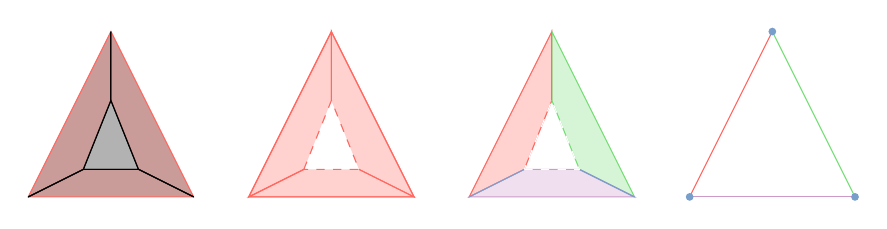
\begin{tikzpicture}[scale=0.7]
  % Coordinates
  \coordinate (A) at (0.00, 0.00);
  \coordinate (B) at (1.50, 3.00);
  \coordinate (C) at (3.00, 0.00);
  \coordinate (D) at (1.00, 0.50);
  \coordinate (E) at (2.00, 0.50);
  \coordinate (F) at (1.50, 1.75);
  \coordinate (J) at (4.00, 0.00);
  \coordinate (K) at (5.50, 3.00);
  \coordinate (L) at (7.00, 0.00);
  \coordinate (M) at (5.00, 0.50);
  \coordinate (N) at (5.50, 1.75);
  \coordinate (O) at (6.00, 0.50);
  \coordinate (G) at (9.00, 0.50);
  \coordinate (H) at (10.00, 0.50);
  \coordinate (I) at (9.50, 1.75);
  \coordinate (P) at (9.50, 3.00);
  \coordinate (Q) at (8.00, 0.00);
  \coordinate (R) at (11.00, 0.00);
  \coordinate (S) at (12.00, 0.00);
  \coordinate (T) at (15.00, 0.00);
  \coordinate (U) at (13.50, 3.00);

  % Drawing
  \filldraw[pastelred, fill=black, fill opacity=0.3] (A) -- (B) -- (C) -- cycle;
  \draw (D) -- (E) -- (F) -- cycle;
  \draw (F) -- (B);
  \draw (A) -- (D);
  \draw (E) -- (C);
  \filldraw[fill=pastelred, fill opacity=0.3] (A) -- (D) -- (F) -- (B);
  \filldraw[fill=pastelred, fill opacity=0.3] (B) -- (F) -- (E) -- (C);
  \filldraw[fill=pastelred, fill opacity=0.3] (C) -- (E) -- (D) -- (A);
  \draw[pastelred] (J) -- (K) -- (L) -- cycle;
  \draw[pastelred, dashed] (M) -- (N) -- (O) -- cycle;
  \filldraw[pastelred, fill=pastelred, fill opacity=0.3] (M) -- (J) -- (K) -- (N);
  \filldraw[pastelred, fill=pastelred, fill opacity=0.3] (O) -- (L) -- (K) -- (N);
  \filldraw[pastelred, fill=pastelred, fill opacity=0.3] (G) -- (Q) -- (P) -- (I) -- cycle;
  \filldraw[pastelred, fill=pastelred, fill opacity=0.3] (M) -- (J) -- (L) -- (O);
  \filldraw[pastelgreen, fill=pastelgreen, fill opacity=0.3] (R) -- (H) -- (I) -- (P) -- cycle;
  \filldraw[pastelviolet, fill=pastelviolet, fill opacity=0.3] (Q) -- (R) -- (H) -- (G) -- cycle;
  \draw[pastelblue] (I) -- (P);
  \draw[pastelblue] (H) -- (R);
  \draw[pastelblue] (G) -- (Q);
  \draw[pastelred] (S) -- (U);
  \draw[pastelgreen] (T) -- (U);
  \draw[pastelviolet] (S) -- (T);
  \fill[pastelblue] (S) circle (2pt);
  \fill[pastelblue] (T) circle (2pt);
  \fill[pastelblue] (U) circle (2pt);
  \draw[white,dashed] (G) -- (G) -- (H) -- (I) -- cycle;
\end{tikzpicture}
\caption{A simplicial up-reduction $\Delta_2\upred\partial\Delta_2$. In order, $\Delta_2$, the domain of the map, a coloring of the domain and the codomain showing what maps to what.}
\end{figure}
\end{proof}

\begin{proposition}
    The class of convex polyhedra and the class of PL-manifolds are not modally definable.
\end{proposition}
\begin{proof}
    Given a convex polyhedron, we may find a non-convex polyhedron with face poset isomorphic to one of its subdivision, just by moving a vertex 
    to the interior of a maximal face.
    This means that we found a non-convex polyhedron that validates and refutes all the formulas that the original did.

    PL-manifolds (in the sense of \cite{Dekker}\textbf{3}) are even simpler, as they're not closed under disjoint unions.
\end{proof}

\section{Open questions}
\subsection{A refinement of GTKP}
The result we have spent the most time trying to obtain is the following refinement:
\begin{conjecture}
    A class of compact polyhedra is modally definable if and only if
    it is closed under finite disjoint unions and simplicial up-reductions.
\end{conjecture}

The procedure we have in mind to prove the equivalence between the current result
and the one above is the following:
\begin{itemize}
    \item Consider the face up-reduction $f:P\fupred Q$ realized as $f:P\upred [L]$;
    \item Realize $f$ as a map $\tilde{f}:[K]\upred [L]$;
    \item Construct an up-reduction $\tilde{g}:K\upred L$ ``informed by $\tilde{f}$''
    that is an up-reduction and a map of simplicial complexes;
    \item Realize $\tilde{g}$ as a simplicial up-reduction $g:P\upred Q$.
\end{itemize}
If $\tilde{f}$ were (or were densely contained in) a map of (abstract) simplicial complexes, rather than merely one of posets, our work would be done: it is possible to realize any map of ASCs as a simplicial map of their polyhedra.

In general, though, this is not the case. Consider $P$ to be three segments and $Q$ the triangle (the boundary of the $2$-simplex):

\begin{figure}[H]
  \centering
  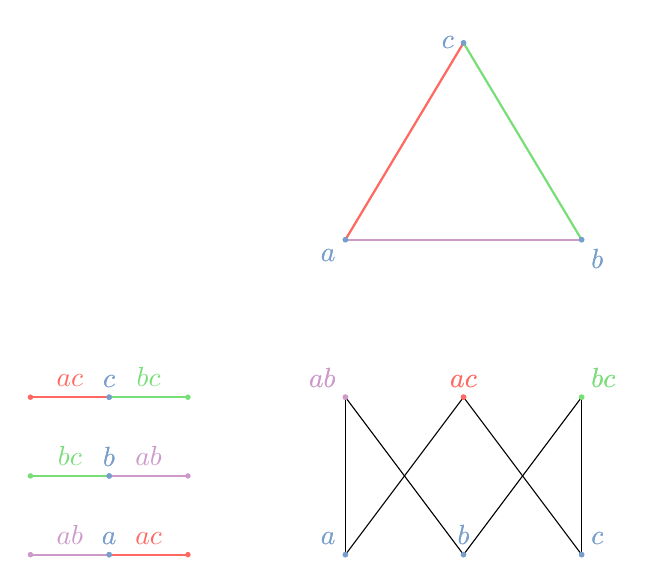
\begin{tikzpicture}[scale=1]
  % Coordinates
  \coordinate (A) at (0.00, 0.00);
  \coordinate (B) at (2.00, 0.00);
  \coordinate (D) at (0.00, 1.00);
  \coordinate (E) at (2.00, 1.00);
  \coordinate (F) at (0.00, 2.00);
  \coordinate (J) at (4.00, 0.00);
  \coordinate (K) at (4.00, 2.00);
  \coordinate (L) at (5.50, 2.00);
  \coordinate (M) at (7.00, 0.00);
  \coordinate (N) at (7.00, 2.00);
  \coordinate (O) at (5.50, 0.00);
  \coordinate (P) at (4.00, 4.00);
  \coordinate (Q) at (7.00, 4.00);
  \coordinate (R) at (5.50, 6.50);
  \coordinate (G) at (2.00, 2.00);
  \coordinate (H) at (1.00, 2.00);
  \coordinate (I) at (1.00, 1.00);
  \coordinate (C) at (1.00, 0.00);

  % Drawing
  \draw (A) -- (B);
  \draw (D) -- (E);
  \draw (F) -- (G);
  \draw (J) -- (K);
  \draw (J) -- (L);
  \draw (L) -- (M);
  \draw (M) -- (N);
  \draw (K) -- (O);
  \draw (O) -- (N);
  \draw[gray] (P) -- (Q) -- (R) -- cycle;
  \draw[pastelred, thick] (F) -- node[above, text=pastelred, midway] {$ac$} (H);
  \draw (H) -- (G);
  \draw[pastelgreen, thick] (H) -- node[above, text=pastelgreen, midway] {$bc$} (G);
  \draw[pastelviolet, thick] (I) -- node[above, text=pastelviolet, midway] {$ab$} (E);
  \draw[pastelred, thick] (C) -- node[above, text=pastelred, midway] {$ac$} (B);
  \draw[pastelviolet, thick] (A) -- node[above, text=pastelviolet, midway] {$ab$} (C);
  \draw[pastelgreen, thick] (D) -- node[above, text=pastelgreen, midway] {$bc$} (I);
  \draw[pastelviolet,thick] (P) -- (Q);
  \draw[pastelred, thick] (P) -- (R);
  \fill[pastelred] (B) circle (1pt);
  \draw[pastelgreen, thick] (R) -- (Q);
  \fill[pastelviolet] (A) circle (1pt);
  \fill[pastelgreen] (D) circle (1pt);
  \fill[pastelviolet] (E) circle (1pt);
  \fill[pastelred] (F) circle (1pt);
  \fill[pastelblue] (J) circle (1pt);
  \node[above left, pastelblue] at (J) {$a$};
  \fill[pastelviolet] (K) circle (1pt);
  \node[above left, pastelviolet] at (K) {$ab$};
  \fill[pastelred] (L) circle (1pt);
  \node[above, pastelred] at (L) {$ac$};
  \fill[pastelblue] (M) circle (1pt);
  \node[above right, pastelblue] at (M) {$c$};
  \fill[pastelgreen] (N) circle (1pt);
  \node[above right, pastelgreen] at (N) {$bc$};
  \fill[pastelblue] (O) circle (1pt);
  \node[above, pastelblue] at (O) {$b$};
  \fill[pastelblue] (P) circle (1pt);
  \node[below left, pastelblue] at (P) {$a$};
  \fill[pastelblue] (Q) circle (1pt);
  \node[below right, pastelblue] at (Q) {$b$};
  \fill[pastelblue] (R) circle (1pt);
  \node[left, pastelblue] at (R) {$c$};
  \fill[pastelgreen] (G) circle (1pt);
  \fill[pastelblue] (H) circle (1pt);
  \node[above, pastelblue] at (H) {$c$};
  \fill[pastelblue] (I) circle (1pt);
  \node[above, pastelblue] at (I) {$b$};
  \fill[pastelblue] (C) circle (1pt);
  \node[above, pastelblue] at (C) {$a$};
  \fill[pastelblue] (J) circle (1pt);
  \node[above left, pastelblue] at (J) {$a$};
  \fill[pastelviolet] (K) circle (1pt);
  \node[above left, pastelviolet] at (K) {$ab$};
  \fill[pastelred] (L) circle (1pt);
  \node[above, pastelred] at (L) {$ac$};
  \fill[pastelblue] (M) circle (1pt);
  \node[above right, pastelblue] at (M) {$c$};
  \fill[pastelgreen] (N) circle (1pt);
  \node[above right, pastelgreen] at (N) {$bc$};
  \fill[pastelblue] (O) circle (1pt);
  \node[above, pastelblue] at (O) {$b$};
  \fill[pastelblue] (P) circle (1pt);
  \node[below left, pastelblue] at (P) {$a$};
  \fill[pastelblue] (Q) circle (1pt);
  \node[below right, pastelblue] at (Q) {$b$};
  \fill[pastelblue] (R) circle (1pt);
  \node[left, pastelblue] at (R) {$c$};
  \fill[pastelblue] (H) circle (1pt);
  \node[above, pastelblue] at (H) {$c$};
  \fill[pastelblue] (I) circle (1pt);
  \node[above, pastelblue] at (I) {$b$};
  \fill[pastelblue] (C) circle (1pt);
  \node[above, pastelblue] at (C) {$a$};
\end{tikzpicture}
\caption{An example of a face up-reduction that does not come from a simplicial up-reduction}
\end{figure}

The Hasse diagram (bottom right) is $L$; the three segments are $P$, and the triangle is $Q$. The map is indicated by the coloring.

One can check that it is a p-morphism, but clearly not a map of simplicial complexes, since the images of the vertices are not themselves vertices.

\subsection{The precompact case}

How do things change if we allow open polyhedra? We gain access to generated subframes, but the relationship between polyhedra and simplicial complexes becomes looser:

Consider the poset consisting of a single point: it is the poset of the maximal face of any simplex.

Moreover, even if we try to circumvent this problem by considering the closure of a face --- which is indeed a simplicial complex --- we can find cases where the combinatorial description fails to be PL-invariant.

For example, consider the disjoint union of two triangles:
\begin{figure}[H]
  \centering
  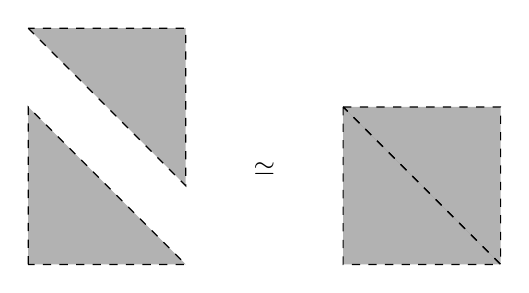
\begin{tikzpicture}[scale=1]
  % Coordinates
  \coordinate (A) at (0.00, 0.00);
  \coordinate (B) at (0.00, 2.00);
  \coordinate (C) at (2.00, 0.00);
  \coordinate (D) at (0.00, 3.00);
  \coordinate (E) at (2.00, 1.00);
  \coordinate (F) at (2.00, 3.00);
  \coordinate (G) at (3.00, 1.01);
  \coordinate (H) at (4.00, 2.00);
  \coordinate (I) at (4.00, 0.00);
  \coordinate (J) at (6.00, 0.00);
  \coordinate (K) at (6.00, 2.00);

  % Drawing
  \filldraw[dashed, fill=black, fill opacity=0.3] (A) -- (B) -- (C) -- cycle;
  \filldraw[dashed, fill=black, fill opacity=0.3] (D) -- (E) -- (F) -- cycle;
  \filldraw[dashed, fill=black, fill opacity=0.3] (H) -- (I) -- (J) -- cycle;
  \filldraw[dashed, fill=black, fill opacity=0.3] (H) -- (K) -- (J) -- cycle;
  \node[above, black] at (G) {$\simeq$};
\end{tikzpicture}
\end{figure}

The two objects are PL-homeomorphic, but their simplicial complexes are not.
\subsection{The infinite case}

An interesting question is what happens when we allow arbitrarily large simplicial complexes, both in dimension and in number of simplices: the relevant class is then no longer that of finite transitive frames, but of arbitrary ones.
\begin{itemize}
    \item What is the geometric realization of an arbitrarily large abstract simplicial complex?
    \item What is the ultrafilter extension of an arbitrarily large simplicial complex?
    \item How do we describe such an ultrafilter extension geometrically?
    \item (Abstract) simplicial complexes admit a coalgebraic description: they form a class of $\Pp\circ \Pp$-coalgebras over sets
    (the map $V\to \Pp\Pp(V)$ associates to every point the up-set of simplices containing it).
    Do completeness and definability results in that setting coincide with the usual ones?
\end{itemize}

\subsection{Dual semantics}.
By - equivalently - switching to the dual modal operators ($\blacksquare,\blacklozenge$) or considering the 
semantics of closed subsets / the converse face relation we get that modally definable classes 
are exactly those closed under disjoint unions, subcomplexes and surjective simplicial maps.
The semantics is not the same and probably incompatible with the topological one, thus prompting for 
a completeness result for this semantics.

\nocite{*}
\printbibliography
\end{document}